\documentclass[a4paper,10pt,twocolumn]{article}

\usepackage{inputenc}
\usepackage{float}
\usepackage{fontenc}
\usepackage{textcomp}
\usepackage{amsmath, amssymb}
\usepackage{graphicx}
\usepackage[width = 18cm,height = 22cm,columnsep = 1cm,margin = 2cm]{geometry}
\usepackage[backend=biber,style=authoryear]{biblatex}
\usepackage{aas_macros}
\usepackage{hyperref}
\hypersetup{
	colorlinks=true,
	linkcolor=blue,
	citecolor=blue,
	urlcolor=cyan,
	pdftitle={Sloan Digital Sky Survey Software Development: Week 9 Progress Report},
	pdfpagemode=FullScreen,
}

\bibliography{/home/riley/rproj/reports/w9/bibliography.bib}
\graphicspath{{/home/riley/rproj/reports/w9/images/}}

\title{Sloan Digital Sky Survey Software Development: Week 9 Progress Report}
\author{Riley Thai, Andy Casey (Supervisor)}

\newcommand{\solara}{\texttt{solara}}
\newcommand{\vaex}{\texttt{vaex}}

\begin{document}
\maketitle
\begin{figure*}
	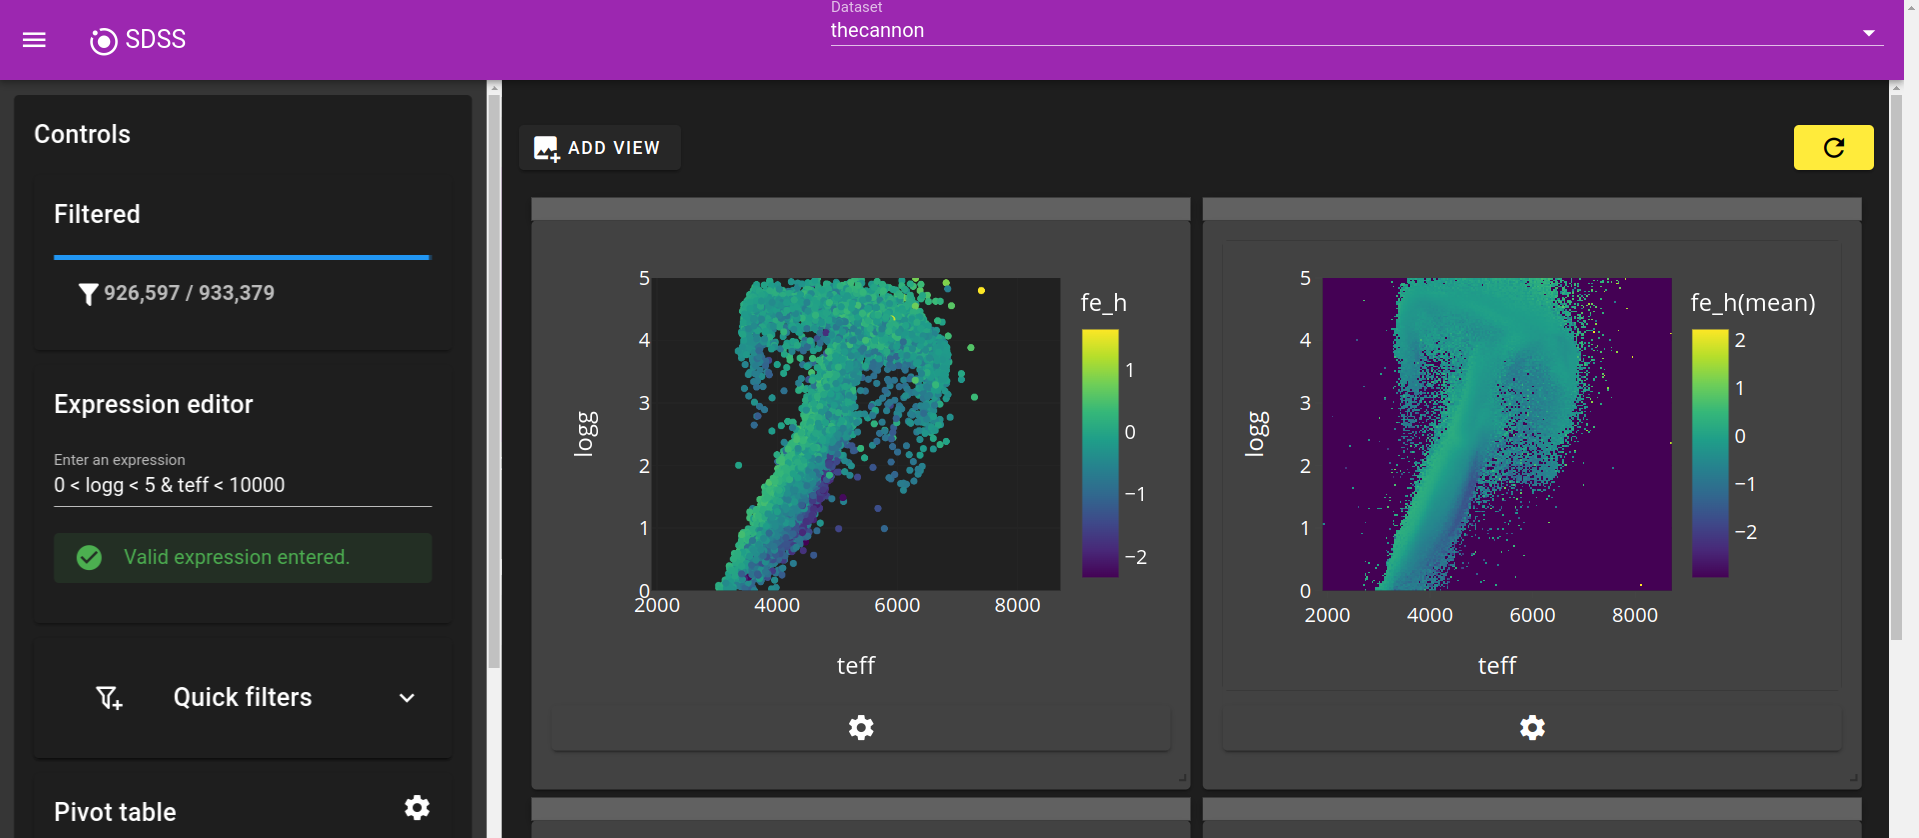
\includegraphics[width=1.0\textwidth]{wholeapp}
	\caption{A full screenshot of the application. Top: the Application bar, where the loaded dataset can be changed, currently viewing data from \emph{The Cannon} \parencite{thecannon}. Left: the sidebar, containing filter controls, such as the expression editor. An expression to filter out values is currently applied. Right: the sticky note layout, showing the scatter and aggregation views, plotting $T_{\mathrm{eff}}$ and $\log g$.}
	\label{fig:wholeapp}
\end{figure*}
\section{Aims and Objectives}
\begin{enumerate}
	\item Develop a out-of-memory web application for multi-dimensional exploration of SDSS-V data.
	\item Work on and contribute to the development of open-source Python libraries.
\end{enumerate}

\section{Background}
The Sloan Digital Sky Survey (SDSS) is one of the largest, longest running, and most used astronomical surveys. Started in 1998 \parencite{dr18}, the SDSS provides all-sky, multi-epoch spectroscopy using telescopes in both hemispheres, providing data used to probe the emergence of chemical elements, reveal the inner mechanisms of stars, and investigate the origin of planets. The latest generation of the survey, SDSS-V, aims to conduct the first homogeneous survey using an optical, ultra-wide integral-field spectroscopic map of the interstellar gas, pioneering spectroscopic monitoring and revealing changes on both short and vast timescales \parencite{SDSS2017}. SDSS data over all survey phases has been cited more than 650,000 times over 111,000 refereed papers \parencite{dr18}.

The SDSS has previously offered a simple web application for end users to access, explore, and investigate spectra and other data. However, the fifth generation of the survey now offers a large catalog of stars with complete stellar labels. With a larger set of spectral types explored \parencite{apogee2017}, and an even larger set of stellar labels (Casey et al., in prep), there is a need for a new tool which provides powerful exploration and visualization of large and vast datasets.


\section{VisBoard Development}
The fifth generation of the SDSS now provides complete stellar labels across multiple different pipelines via the Astra framework. This multi-dimensional parameter explorer, or by its less boring name, the \emph{VisBoard}, is a in-development data webapp which will be hosted on SDSS servers, providing both public and proprietary SDSS data to its users for multi-dimensional data exploration via out-of-memory loading and computation using \texttt{vaex}.
\begin{figure}[tp]
	\centering
	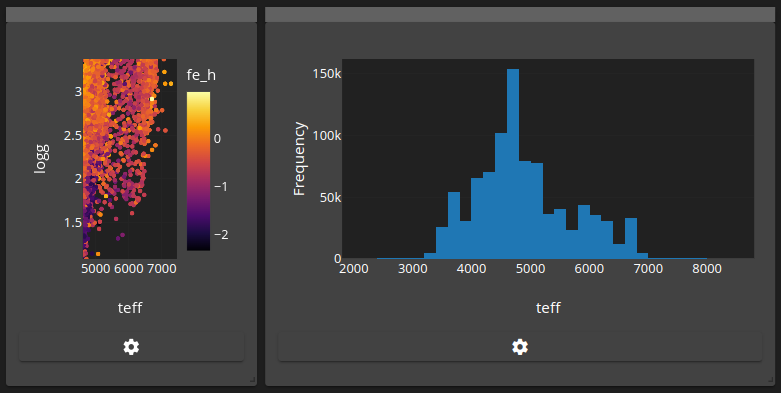
\includegraphics[width=1.0\columnwidth]{layout}
	\caption{A demonstration of the dynamic resizing and draggable view ``notes". The plot objects dynamically resize to fit their container, and can be rearranged and resized by the user with their mouse.}
	\label{fig:layout}
\end{figure}

Since the previous report, updates have been made which primarily improve the user experience (UX) of the software. The utility of the VisBoard has expanded to allow for exploration across a variety of viewing forms through an intuitive user experience. Much like a board of sticky notes, views can be added, removed, and resized at will by the user, whilst applying global filters across the selected dataset. Views themselves are dynamic, rerendering to filter out unnecessary points and saving zoom and pan information for a smoother UX.

In Section \ref{sec:sticky}, we discuss this sticky note layout, and the new skyplot view and dynamic rerendering and filtering in Sections \ref{sec:skyplot} and \ref{sec:rerender} respectively. In Section \ref{sec:datasets}, we describe how the software supports multiple datasets as a proof-of-concept, and discuss future implementations of this functionality. Finally, in Section \ref{sec:other}, we list other additional features added to the software since the last report.

\subsection{Sticky Note Layout}
\label{sec:sticky}
The user can now directly add and remove multiple plotting views of the same time within their display, which can resized with a small handle in the bottom right, and moved via the top grey toolbar, as shown in Figure \ref{fig:wholeapp}. Each plot also dynamically resizes to its containing ``note", which can be seen in Figure \ref{fig:layout}.

Within each view, a plot's individual properties can be changed, such as colorscale, the data to plot, and whether a given axis is flipped and/or logarithmic scale, as shown in Figure \ref{fig:skyplot}.

Each plot (excluding the \emph{aggregation} view) now has a selection option, which allows the user to select certain bins or points, which will then be cross filtered to other open views.

On the scatter plot views, a user can right click on any given star to directly download or view the object's spectra in the browser via \texttt{jdaviz}. Currently, these lead to placeholders, but will eventually be replaced with browser links to the public SDSS data by the ID lookup.

\subsubsection{Skyplot}
\label{sec:skyplot}
New to this format is a scatter plot with a sky projection, herein referred to as a ``\emph{skyplot}". This view was heavily requested by astronomers after consultations and demos. The user can switch between plotting right ascension vs. declination ($\mathrm{RA / DEC} $) or galactic longitude and latitude ($l / b $). Panning the view will accurately map the points according to the projection type, which can be set by the user. The settings menu and skyplot are shown in Figure \ref{fig:skyplot}.


\subsubsection{Dynamic rerendering and filtering}
\label{sec:rerender}
Another new feature is the adaptive rerendering of Plotly's \texttt{FigureWidget} objects, which consists of two parts:
\begin{enumerate}
	\item Rerendering the plot with the same zoom and pan settings after a parameter change.
	\item Filtering the dataset in the Scatter object views (\emph{skyplot} + \emph{scatter}) to the ranges of the zoomed plot in real time.
\end{enumerate}

Previously, the plot would forcibly reset after any parameter change, such as changing the colorscale or binning type, which led to a disorienting UX that required the user to continuously redo their zoom/pan actions after parameter changes. Now, the plot continuously saves the visible x/y ranges, and calls upon them when plotting, only resetting it if the x/y data or plotting scale changes.

The other consequence of saving the relayout information is that we can directly filter the dataset to only include data inside the visible range, which allows the user to see more points after performing zoom or pan operations, bypassing the overplotting limitations of Plotly's memory-heavy scatter points. This is similar in function to Holoview's \texttt{DataShader} \parencite{holoviews}, although we do not rasterize the data prior to plotting.

\subsection{Multiple Datasets}
\label{sec:datasets}
Within the top left of the application, the user can now directly select the Astra pipeline from which to access data from (see top of Figure \ref{fig:wholeapp}).

Currently, this is implemented as a proof-of-concept feature, with the goal being to allow a user to select multiple pipeline datasets simultaneously, and apply unique filters and expressions directly between them or across all of them, and even their own given subsets.

The user's subset of the chosen dataset can also be directly downloaded, based on their chosen filters.
\begin{figure}[tp]
	\centering
	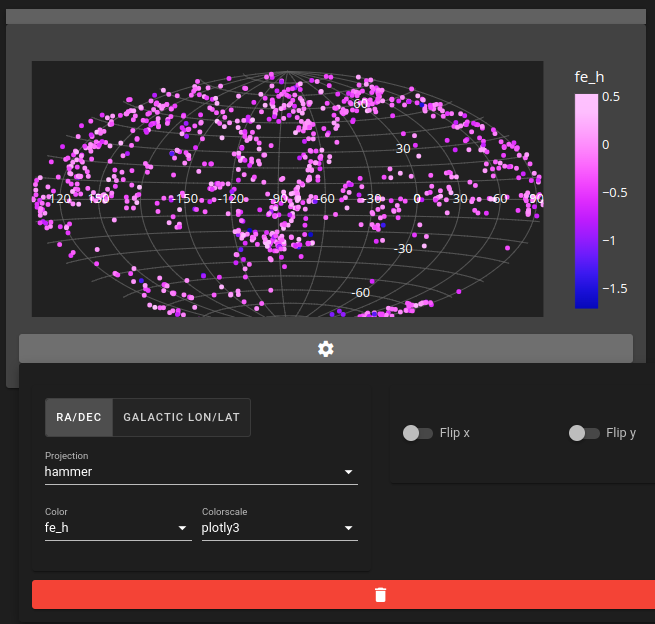
\includegraphics[width=1.0\columnwidth]{skyplot}
	\caption{Top: the \emph{skyplot} view, showing right ascension (RA) against declination (DEC), and colored by metallicity $\mathrm{[Fe / H]}$ across a Hammer projection. Bottom: the settings menu of the skyplot view, where the coordinates, projection type, color values, colorscale, and axes flips can be changed by the user.}
	\label{fig:skyplot}
\end{figure}

\subsection{Other features}
\label{sec:other}
\begin{itemize}
	\item Expression editor updates, as shown in the left of Figure \ref{fig:wholeapp}.
	      \begin{itemize}
		      \item Added the ability to type expressions without brackets.
		      \item Added functionality to type 3-part expressions (i.e. $400 < x \le 3000$)
		      \item Expression editor returns a more descriptive error message.
		      \item Expression editor catches expressions which reduce the dataset to a pointlessly low length.
	      \end{itemize}
	\item Added a Dark theme to the UI, matching the SDSS front-end framework \texttt{zora}.
	\item Added a Quick Filters menu for common filters (i.e.\ good results only)
	\item Added point-hover information to all views.
	\item Added selection filtering functionality to \emph{histogram} and \emph{scatter} plots.
	\item Added ascending/descending sorting options to the Table View card.
	\item (Partly) fixed a bug relating to CPU stride in \texttt{vaex}.
	\item Removed a defunct setting in Plotly.py's \texttt{imshow} plots.
\end{itemize}
\section{Difficulties encountered}
\begin{enumerate}
	\item \textbf{\texttt{vaex} and \texttt{solara} documentation is often incomplete.}
	      \begin{itemize}
		      \item Continuously, I found several API methods and hooks within the source code that were not apparent on the documentation.
		      \item This is common throughout open-source development, due to its decentralized nature, but I will also endeavour to ensure I properly document my work.
	      \end{itemize}
	      \item\textbf{Plotly's \texttt{FigureWidget} is very difficult to debug.}
	      \begin{itemize}
		      \item Spanning across 3 codebases and over 60,000 lines of code, the \texttt{FigureWidget} has been difficult to debug.
		      \item The \texttt{FigureWidget} doesn't resize its height to its container, even though it's specified in CSS that it should.
		            \begin{itemize}
			            \item I have no idea why, even after combing the codebase and testing different resize managers.
			            \item It also does not help that I am not fluent in Jupyter widget libraries, Typescript, or Javascript.
		            \end{itemize}
		      \item Solving this problem is out of scope for the project's timescale, so the views are height-locked until this is fixed.
	      \end{itemize}
\end{enumerate}
\section{Future plans}
\begin{enumerate}
	\item \textbf{Add dynamic filtering to the \emph{skyplot} view.}
	      \begin{itemize}
		      \item Due to the difference in relayout callback information, it was not simply plug and play to implement the routine.
		      \item It wasn't finished prior to writing this report, but the logic is sorted already and just needs to be implemented.
	      \end{itemize}
	      \item\textbf{Develop a \texttt{Singularity} container for shared development.}
	      \begin{itemize}
		      \item The Data Visualization group within the SDSS Collaboration will soon be granted access to a virtual machine (VM) for testing and developing applications.
		      \item Members of the collaboration are interested in providing feedback and testing the application, and have suggested using \texttt{Singularity} \parencite{singularity} as the portable app-container for the development workflow.
	      \end{itemize}
	\item \textbf{Expand upon dataset functionality.}
	      \begin{itemize}
		      \item As described in Section \ref{sec:datasets}, I plan to expand upon the dataset functionality.
		      \item The exact implementation of this feature and method depends on how data will be stored across different access methods, which is yet to be decided.
		            \begin{itemize}
			            \item i.e.\ will it be a single file containing all the data? Will it be constantly updated? Or will there be multiple files that must be combined?
		            \end{itemize}
	      \end{itemize}
	\item \textbf{Expand upon \texttt{vaex} methods.}
	      \begin{itemize}
		      \item \texttt{vaex}'s features to provide lazy, out-of-memory computations is of interest for features in the exploration application.
		      \item I plan to add features that allow the user to analyse different subsets based on a \texttt{groupby} routine, and create virtual columns that are based on lazy computations on data from other columns (see \href{https://vaex.io/docs/tutorial.html#Virtual-columns}{\texttt{vaex}'s documentation} for further reading).
	      \end{itemize}
\end{enumerate}

\printbibliography

\end{document}


